\documentclass{article}
\usepackage{hw_style}
\usepackage{enumerate}
\usepackage{graphicx}
\usepackage{verbatim}

% Homework Specific Information
\newcommand{\hmwkTitle}{Homework \#1}
\newcommand{\hmwkDueDate}{}
\newcommand{\hmwkAuthorName}{Kurt Rudolph}%Name:
\newcommand{\hmwkNetID}{rudolph9}%your netid
\newcommand{\hmwkNotes}{}%I worked with...

\newcommand{\hmwkSubTitle}{}
\newcommand{\hmwkClass}{CS 425}
\newcommand{\hmwkClassTime}{Tue, Thir 2:00PM - 3:15PM}
\newcommand{\hmwkClassInstructor}{Nikita Borisov}

\begin{document}
\begin{spacing}{1.1}
\maketitle
%=============================Problem1==========================%	
\newpage
\begin{homeworkProblem}
	Ring heart-beating may not detect simultaneous multiple failures of processors.
	\begin{enumerate}[(1)]
		\item What is the maximum number of simultaneous processor failures that can be detected by ring heart-beating protocol?
			\begin{homeworkSection}{Solution}
		
			\end{homeworkSection}
		\item Modify the ring heart-beating protocol to detect up to 4 simultaneous processor failures.  
			\begin{homeworkSection}{Solution}
		
			\end{homeworkSection}
	\end{enumerate}
\end{homeworkProblem}
%=============================Problem2==========================%
\newpage
\begin{homeworkProblem}
	(Problem 2.14 from the book) Consider two communication services for use in asynchronous distributed systems. In service A, messages may be lost, duplicated or delayed and checksums apply only to headers. In service B, messages may be lost, delayed, or delivered too fast for the recipient to handle them, but those that are delivered arrive with the correct contents.
	\begin{enumerate}[(1)]
		\item Describe the classes of failure exhibited by each service.
			\begin{homeworkSection}{Solution}
		
			\end{homeworkSection}
		\item Can service B be described as a reliable communication service?
			\begin{homeworkSection}{Solution}
		
			\end{homeworkSection}
	\end{enumerate}
\end{homeworkProblem}
%=============================Problem3==========================%
\newpage	
\begin{homeworkProblem}
	P1, P2, P3, and P4 are four processes. Write down the vector logical timestamps in the boxes attached to each event.
	\\ 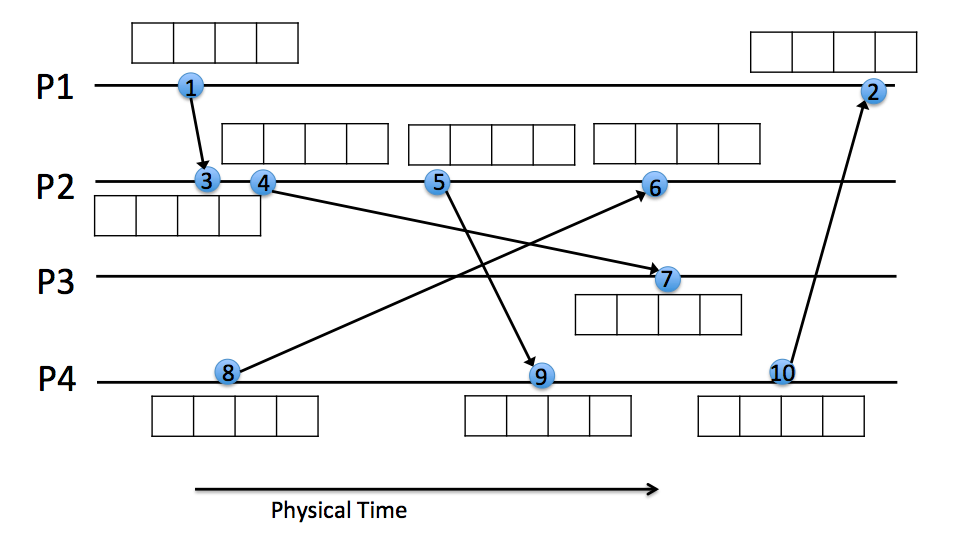
\includegraphics[width=\linewidth]{prob3.png}
	\begin{homeworkSection}{Solution}
		
	\end{homeworkSection}
\end{homeworkProblem}
%=============================Problem4==========================%
\newpage
\begin{homeworkProblem}
	Process P3 initiates the snapshot algorithm. The black arrows are messages sent and received. The red arrows are marker messages. Find out the consistent cut corresponding to this global snapshot and mark the states of each process and channel.
	\\ 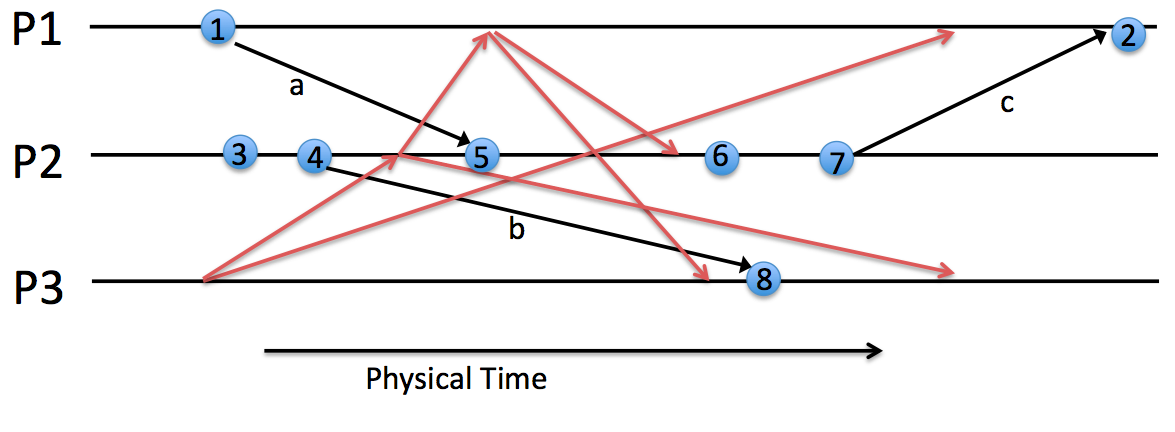
\includegraphics[width=\linewidth]{prob4.png}
	\begin{homeworkSection}{Solution}
		
	\end{homeworkSection}
\end{homeworkProblem}
%=============================Problem5==========================%
\newpage
\begin{homeworkProblem}
	Consider multicast messages sent and received using the order illustrated below. What ordering does this example follow? (a) FIFO (b) Causal (c) Total (d) FIFO-Total (e) Causal-Total.
	\\ 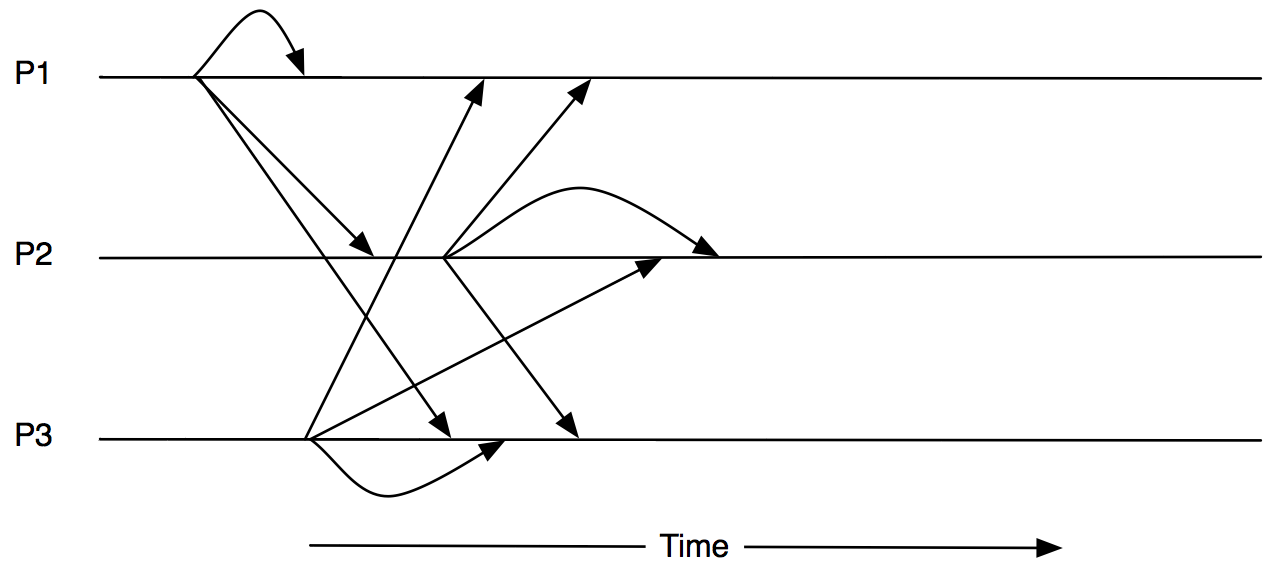
\includegraphics[width=\linewidth]{prob5.png}
	\begin{homeworkSection}{Solution}
		
	\end{homeworkSection}
\end{homeworkProblem}
%=============================Problem6==========================%
\newpage
\begin{homeworkProblem}
The figure below illustrates message flow in a multicast group that uses the Isis total ordering algorithm. Processes P1, P2, P3 each multicast message A,B,C, respectively. The figure shows the transmission and reception times of each initial message transmission (i.e., step 1 of the Isis algorithm).
	\\ 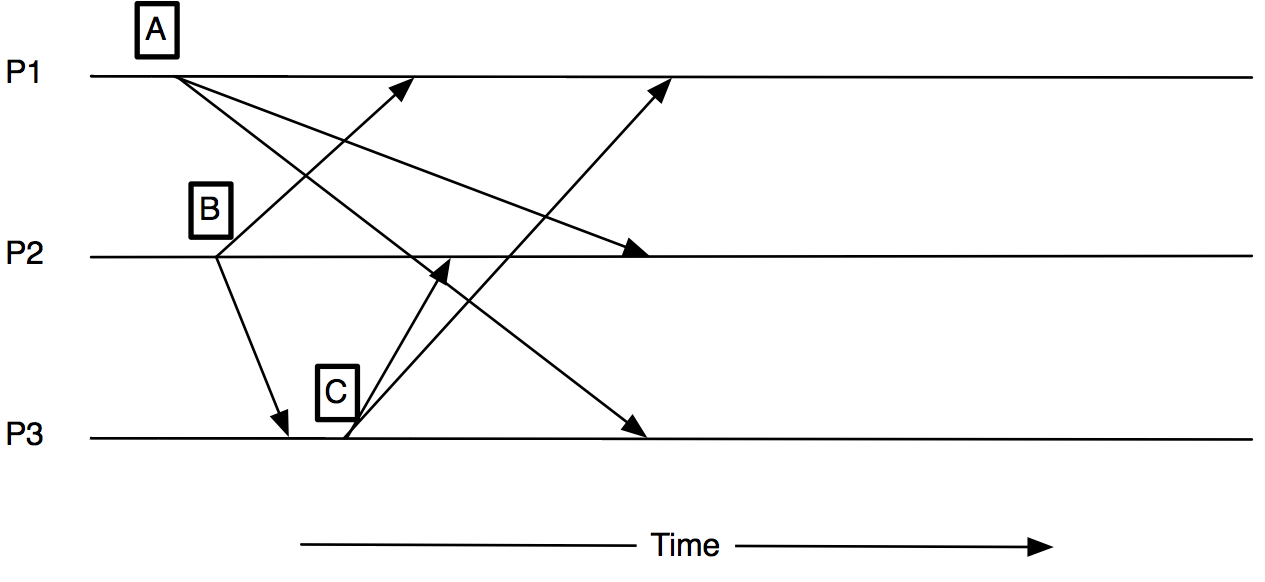
\includegraphics[width=\linewidth]{prob6.png}
	\begin{enumerate}[(a)]
		\item Show the priority queues at each process at the completion of the messages shown and the proposed priority that each process assigns to each message.
			\begin{homeworkSection}{Solution}
		
			\end{homeworkSection}
		\item What is the (total) order that the messages will be delivered in?
			\begin{homeworkSection}{Solution}
		
			\end{homeworkSection}
		\item Prove or disprove: \emph{The Isis total ordering system always produces a FIFO total order.}
			\begin{homeworkSection}{Solution}
		
			\end{homeworkSection}
	\end{enumerate}
\end{homeworkProblem}

\end{spacing}
\end{document}


\begin{comment}%==========================================================
%=============================Problemi==========================%	
\begin{homeworkProblem}
	
	\begin{homeworkSection}{Solution}
		
	\end{homeworkSection}
\end{homeworkProblem}
%=============================Problemi==========================%	
\begin{homeworkProblem}
	
	\begin{enumerate}[(a)]
		\item 
			\begin{homeworkSection}{Solution}
		
			\end{homeworkSection}
	\end{enumerate}
\end{homeworkProblem}
%=============================Problemi==========================%	
\begin{homeworkProblem}
	{\bf }	
	\begin{homeworkSection}{Solution}
		
	\end{homeworkSection}
\end{homeworkProblem}
%=============================Problemi==========================%	
\newpage
\begin{homeworkProblem}
	{\bf  }	
	\begin{enumerate}[(a)]
		\item 
			\begin{homeworkSection}{Solution}
		
			\end{homeworkSection}
	\end{enumerate}
\end{homeworkProblem}
%=============================Problemi=========================%
\newpage
\begin{homeworkProblem}
	
	\begin{homeworkSection}{Solution}
		
	\end{homeworkSection}
\end{homeworkProblem}

\end{comment}%=========================================================
















